% Results-only version of breaking_TRS.tex for sharing; same figs/ and tables/.
\documentclass[aps,prb,twocolumn,superscriptaddress,nofootinbib]{revtex4-2}

\usepackage{amsmath, amssymb, physics}
\usepackage{bm}
\usepackage{graphicx}
\usepackage[hidelinks]{hyperref}

\newcommand{\bk}{\bm{k}}
\newcommand{\bq}{\bm{q}}
\newcommand{\br}{\bm{r}}

\begin{document}

\title{Seeing chiral superconductivity in QPI: results}

\date{\today}

\maketitle

\section{Setup}

Nearest-neighbour triangular lattice, single impurity, broadening $\Gamma = 10^{-3}$, $V_0 = 0.1$, $|\Delta| = 0.1$ (units of the hopping), $240 \times 240$ $\bk$-mesh, $120 \times 120$ $\bq$-mesh.
Spinful Nambu basis $(c_{\bk\uparrow}, c_{\bk\downarrow}, c^\dagger_{-\bk\uparrow}, c^\dagger_{-\bk\downarrow})$; the LDOS is resolved by spin, $\delta\rho_\mu$ with $\mu \in \{0, x, y, z\}$.
Born approximation unless stated, with a Gaussian momentum cutoff $e^{-q^2/q_0^2}$ ($q_0$ in units of $|\bm b_1|$).
Every $\delta\rho(\bq)$ is projected onto the irreps of $C_{6v}$, with weight $\sum|f_\nu|^2 / \sum|f|^2$.
Pairings: $s$, extended $s$, $d_{x^2-y^2}$ (nematic) and $d+id$ (chiral), singlet, at $\omega = 0$ and $\omega_2$ just below the gap edge ($\omega_2 = 0.15$ for the nodal $d_{x^2-y^2}$ state).
Each panel is normalised to its own maximum, given below it.
Table~\ref{tab:cases} summarises all cases.

\begin{table*}[tp]
    \caption{Irreps of the spin-resolved QPI $\delta\rho_\mu(\bq)$ for each system, impurity and pairing. $0$ means the channel vanishes.
    Each pairing is labelled by its own $C_{6v}$ irrep, which for FRG includes spin-symmetric pairings allowed under Rashba SOC.
    Each entry combines $\omega = 0$ and $\omega_2$.
    All $A_1$-irrep impurities hold both in the Born approximation and with the full $T$-matrix. The $\dagger$ notes where the QPI is instead zero in the Born approximation at $\omega=0$. The $A_2$ impurity case was only calculated in the Born approximation.
    ``Im'' marks a channel that is purely imaginary in $\bq$-space; all others are real.
    Irreps with weight below $10^{-3}$ are omitted.
    The last column gives the figures in which that case's QPI is plotted.}
    \label{tab:cases}
    \begin{ruledtabular}
    \begin{tabular}{lllllllll}
        System & Impurity & Pairing & $\omega_2$ & $\delta\rho_0$ & $\delta\rho_x$ & $\delta\rho_y$ & $\delta\rho_z$ & Fig. \\
        \hline
                no SOC & A1 & $A_1$: $s$ & 0.0980 & $A_1$ & $0$ & $0$ & $0$ & \ref{fig:nosoc_A1}(a) \\
         &  & $A_1$: ext.\ $s$ & 0.0098 & $A_1$ & $0$ & $0$ & $0$ & \ref{fig:nosoc_A1}(b) \\
         &  & $E_2$: $d+id$ & 0.2142 & $A_1$ & $0$ & $0$ & $0$ & \ref{fig:nosoc_A1}(c) \\
         &  & $E_2$: $d_{x^2-y^2}$ & 0.1500 & $A_1$ + $E_2$ & $0$ & $0$ & $0$ & \ref{fig:nosoc_A1}(d) \\
        \cline{2-9}
         & A2 & $A_1$: $s$ & 0.0980 & $0$ & $0$ & $0$ & $0$ & -- \\
         &  & $A_1$: ext.\ $s$ & 0.0098 & $0$ & $0$ & $0$ & $0$ & -- \\
         &  & $E_2$: $d+id$ & 0.2142 & $A_1$$^\dagger$ & $0$ & $0$ & $0$ & \ref{fig:nosoc_A2} \\
         &  & $E_2$: $d_{x^2-y^2}$ & 0.1500 & $0$ & $0$ & $0$ & $0$ & -- \\
        \hline
        Rashba & A1 & $A_1$: $s$ & 0.0980 & $A_1$ & $0$ & $0$ & $0$ & \ref{fig:rashba_nonchiral}(a) \\
         &  & $A_1$: ext.\ $s$ & 0.0187 & $A_1$ & $0$ & $0$ & $0$ & \ref{fig:rashba_nonchiral}(b) \\
         &  & $E_2$: $d+id$ & 0.2095 & $A_1$ & $\mathrm{Im}$: $E_1$$^\dagger$ & $\mathrm{Im}$: $E_1$$^\dagger$ & $A_1$$^\dagger$ & \ref{fig:dpid_compare} \\
         &  & $E_2$: $d_{x^2-y^2}$ & 0.1500 & $A_1$ + $E_2$ & $0$ & $0$ & $0$ & \ref{fig:rashba_nonchiral}(c) \\
        \hline
        Rashba--Hubbard & A1 & $A_1$: $U{=}0, V{=}0.9$ & 0.0761 & $A_1$ & $0$ & $0$ & $0$ & \ref{fig:frg_nonchiral} \\
        (FRG) &  & $E_2$: $U{=}8, V{=}0$, $\chi{=}+1$ & 0.0846 & $A_1$ & $\mathrm{Im}$: $E_1$ & $\mathrm{Im}$: $E_1$ & $A_1$ & \ref{fig:frg_spin} \\

    \end{tabular}
    \end{ruledtabular}
\end{table*}

\section{No spin-orbit coupling}

\paragraph{Scalar ($A_1$) impurity.}
All spin channels vanish.
$\delta\rho$ is purely $A_1$ for $s$, extended $s$ and $d+id$; only the nematic $d_{x^2-y^2}$ state has an $E_2$ part (Fig.~\ref{fig:nosoc_A1}).
A scalar impurity sees nematicity but not chirality.

\begin{figure*}[tp]
    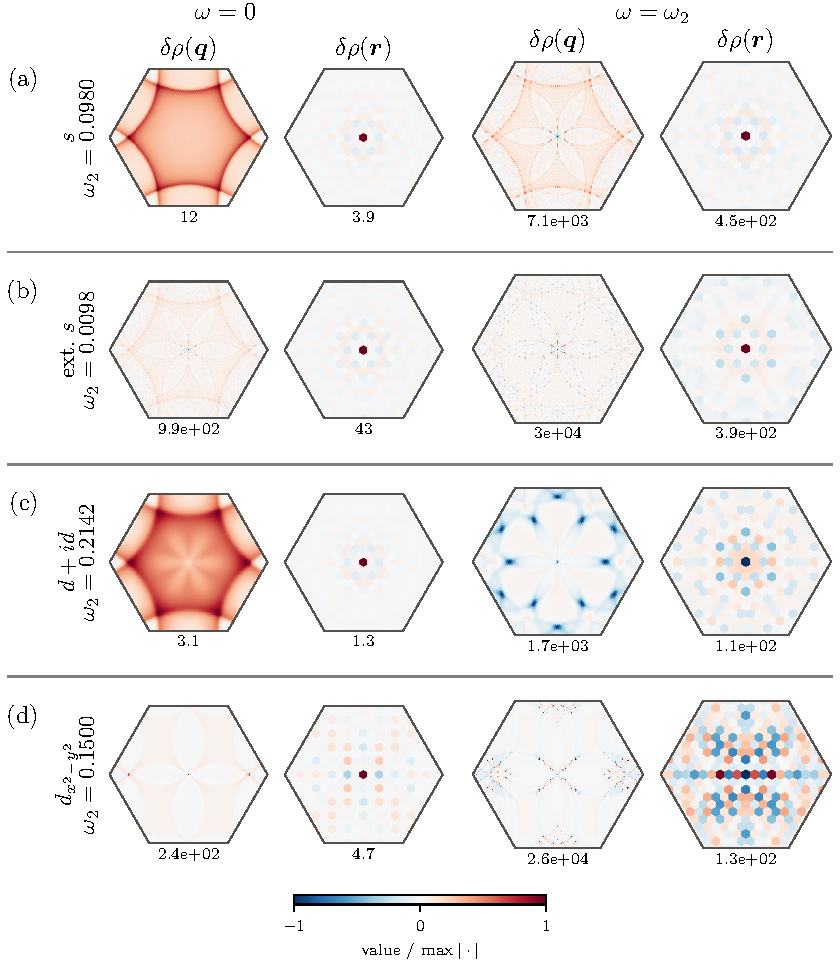
\includegraphics[width=0.8\textwidth]{figs/nosoc_A1imp_all.pdf}
    \caption{No SOC, scalar ($A_1$) impurity, $q_0 = |\bm b_1|$.
    Rows (a)--(d): $s$, extended $s$, $d+id$ and $d_{x^2-y^2}$ pairing.
    Columns: $\operatorname{Re}\delta\rho(\bq)$ and $\delta\rho(\br)$ at $\omega = 0$, then the same at $\omega_2$, which is given on each row.
    $\operatorname{Im}\delta\rho(\bq)$ and all spin channels vanish.
    Only the nematic $d_{x^2-y^2}$ state has a component beyond $A_1$, from the $E_2$ irrep, which breaks $C_6$ down to $C_2$.}
    \label{fig:nosoc_A1}
\end{figure*}

\paragraph{$A_2$ impurity.}
$V(\bk, \bk') = i V_0 (\bk \times \bk')_z \, e^{-|\bk - \bk'|^2/q_0^2}$, $q_0 = 20 |\bm b_1|$.
$\delta\rho$ vanishes for every case except $d+id$ at $\omega_2$, where it is purely $A_1$ (Fig.~\ref{fig:nosoc_A2}).

\begin{figure}[tp]
    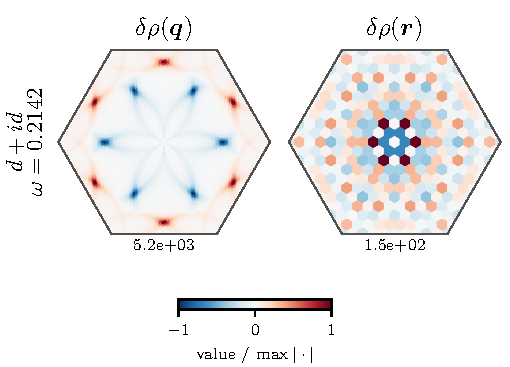
\includegraphics[width=\columnwidth]{figs/nosoc_A2imp_nonzero.pdf}
    \caption{No SOC, $A_2$ impurity, $q_0 = 20|\bm b_1|$: the only non-zero case, $d+id$ at $\omega_2 = 0.2142$, with the panel conventions of Fig.~\ref{fig:nosoc_A1}.
    $\delta\rho$ vanishes identically for $s$, extended $s$ and $d_{x^2-y^2}$ pairing at both frequencies, and for $d+id$ at $\omega = 0$.
    The response is purely $A_1$.}
    \label{fig:nosoc_A2}
\end{figure}

\section{Rashba SOC, ansatz pairings}

$\hat h(\bk) = \varepsilon(\bk) + \alpha\,(\partial_{k_y}\varepsilon\, \sigma_x - \partial_{k_x}\varepsilon\, \sigma_y)$, $\alpha = 0.1$, $\mu = -0.1$, $\hat\Delta = \Psi(\bk)\, i\sigma_y$; scalar impurity.
Bands in Fig.~\ref{fig:bands}.
For $s$, extended $s$ and $d_{x^2-y^2}$ only $\delta\rho_0$ is finite (Fig.~\ref{fig:rashba_nonchiral}).
For $d+id$ at $\omega_2$, all four channels are finite: $\delta\rho_0, \delta\rho_z \in A_1$ and $\operatorname{Im}\delta\rho_{x,y} \in E_1$ (Fig.~\ref{fig:dpid_compare}).
An $A_1$ pattern in $\delta\rho_z$ requires broken time reversal and broken mirrors together, i.e.\ the chiral state.

\begin{figure}[t]
    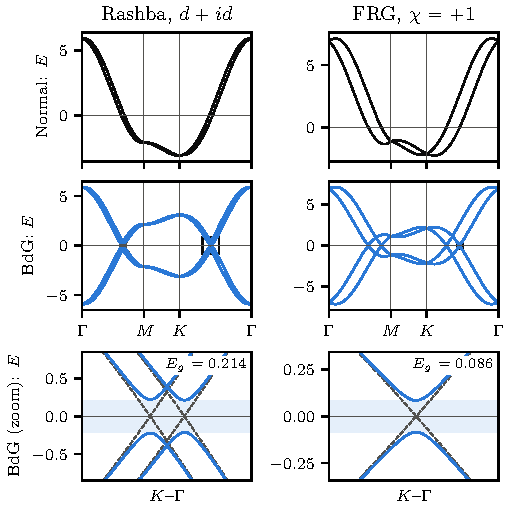
\includegraphics[width=\columnwidth]{figs/bands_combined.pdf}
    \caption{Bands on $\Gamma$--$M$--$K$--$\Gamma$ for the two chiral states.
    Left: Rashba model ($\alpha = 0.1$, $\mu = -0.1$) with $d+id$ singlet pairing, $|\Delta| = 0.1$.
    Right: FRG gap of the Rashba-Hubbard model ($U = 8$, $\alpha = 0.4$, half filling), $\chi = +1$, $\Delta_{\text{rms}} = 0.1$.
    Rows: normal state; BdG bands (solid) with $\pm\varepsilon(\bk)$ (dashed); BdG bands zoomed on the boxed region, the Fermi crossing with the smallest gap on the path.
    The shading marks $|E| < E_g$, with $E_g$ the gap over the whole Brillouin zone.}
    \label{fig:bands}
\end{figure}

\begin{figure*}[tp]
    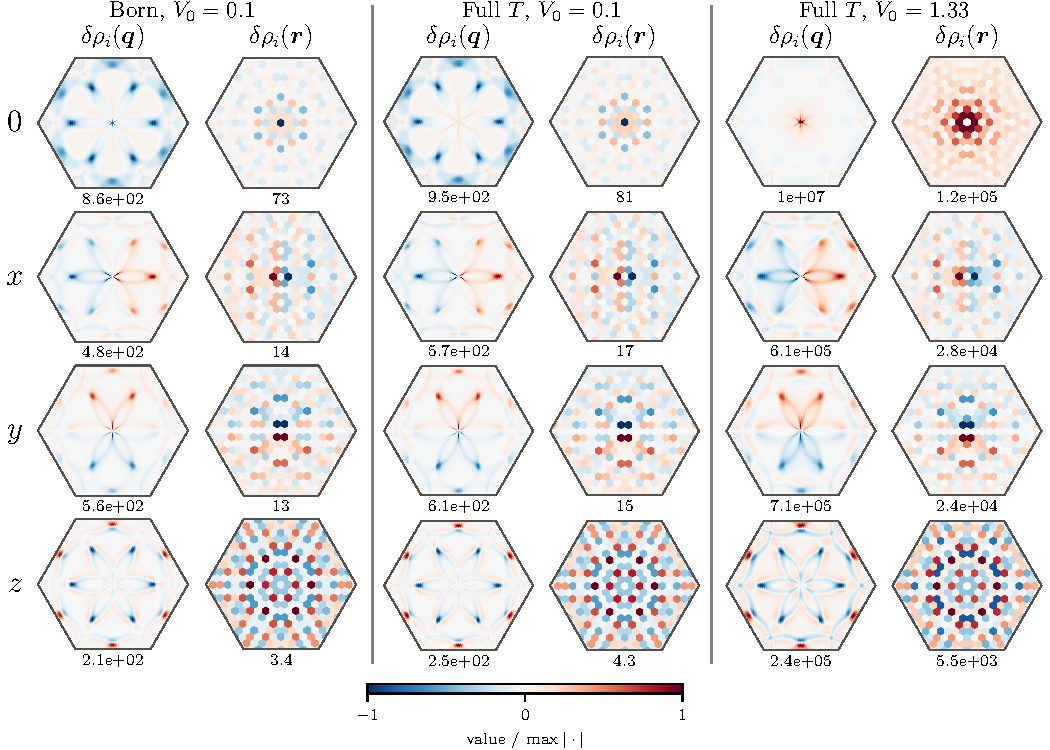
\includegraphics[width=\textwidth]{figs/dpid_compare.pdf}
    \caption{Spin-resolved QPI for the Rashba model with $d+id$ pairing and a scalar impurity, at $\omega_2 = 0.2095$.
    Left: Born approximation, $q_0 = |\bm b_1|$.
    Centre: full $T$-matrix at the same $V_0$.
    Right: full $T$-matrix at the resonance $V_0 = 1.33$ ($\max|\hat T| = 40$).
    Here $\delta\rho_0(\bq)$ is dominated by a broad peak at $\bq = 0$ from the impurity bound state, which hides the scattering pattern of the other two columns; the spin channels keep that pattern.
    The full-$T$ panels have no $q$ cutoff.
    Rows are $i = 0, x, y, z$; the $\bq$-maps show $\operatorname{Im}\delta\rho_i$ for $x, y$ and $\operatorname{Re}\delta\rho_i$ for $0, z$, and the other part vanishes.
    Each panel is normalised to its own maximum, given below it; for the $\bq$-maps this is the maximum over $\bq \neq 0$, so the $\bq = 0$ point saturates.
    The irreps are given in Table~\ref{tab:cases}.}
    \label{fig:dpid_compare}
\end{figure*}

\begin{figure}[tp]
    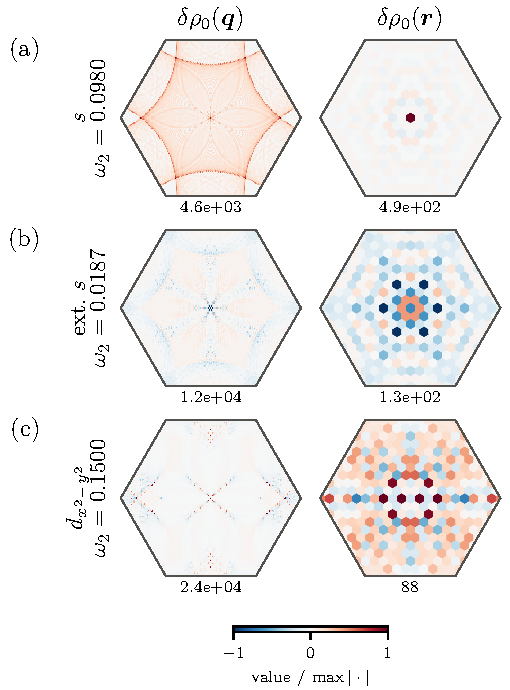
\includegraphics[width=\columnwidth]{figs/rashba_born_nonchiral.pdf}
    \caption{$\operatorname{Re}\delta\rho_0$ for the Rashba model with $s$, extended $s$ and $d_{x^2-y^2}$ pairing, scalar impurity, Born approximation, $q_0 = |\bm b_1|$, each at its $\omega_2$.
    All spin channels vanish.
    Normalisation as in Fig.~\ref{fig:dpid_compare}.}
    \label{fig:rashba_nonchiral}
\end{figure}

\section{Rashba-Hubbard model, FRG pairing}

Leading $\bq = 0$ pairing instability of a divERGe FRG flow at half filling, $\Delta_{\text{rms}} = 0.1$; scalar impurity.
$U = 0$, $\alpha = 0.1$ (non-degenerate): only $\delta\rho_0 \in A_1$ (Fig.~\ref{fig:frg_nonchiral}).
$U = 8$, $\alpha = 0.4$ (two-fold degenerate; chiral combination $(v_0 + i v_1)/\sqrt2$): the ansatz $d+id$ pattern, already finite at $\omega = 0$ (Fig.~\ref{fig:frg_spin}).

\begin{figure*}[tp]
    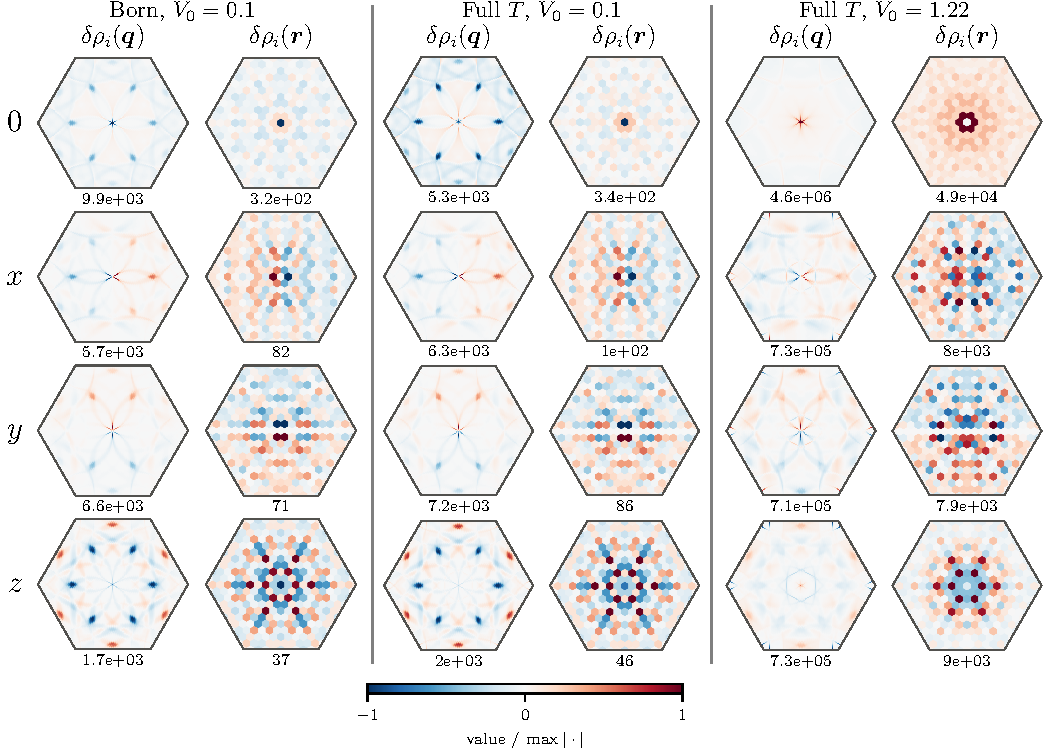
\includegraphics[width=\textwidth]{figs/frg_compare.pdf}
    \caption{Spin-resolved QPI for the chiral FRG state of Fig.~\ref{fig:bands}, scalar impurity, $\omega = 0.0846$.
    Left: Born approximation, $q_0 = |\bm b_1|$.
    Centre: full $T$-matrix at the same $V_0$.
    Right: full $T$-matrix at the resonance $V_0 = 1.22$ ($\max|\hat T| = 12$), the sharpest of the four at this $\omega$; as in Fig.~\ref{fig:dpid_compare}, the bound state dominates $\delta\rho_0$, while the spin channels keep their pattern.
    The full-$T$ panels have no $q$ cutoff.
    Panel conventions as in Fig.~\ref{fig:dpid_compare}; $\delta\rho_z$ is $A_1$ in all three.}
    \label{fig:frg_spin}
\end{figure*}

\begin{figure*}[tp]
    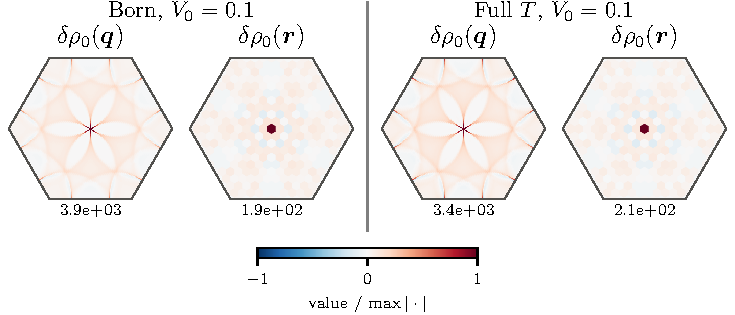
\includegraphics[width=0.7\textwidth]{figs/frg_nonchiral.pdf}
    \caption{$\operatorname{Re}\delta\rho_0$ for the non-chiral FRG state ($U = 0$, $\alpha = 0.1$), scalar impurity, $\omega = 0.0761$, as in Fig.~\ref{fig:frg_spin}.
    All spin channels vanish.
    This state has no impurity bound states, so there is no resonant case.}
    \label{fig:frg_nonchiral}
\end{figure*}

\section{Full $T$-matrix}

Point scalar impurity, no momentum cutoff, $\hat T(\omega) = [1 - \hat V \hat G_{\text{loc}}(\omega)]^{-1} \hat V$ with $\hat V = V_0 \tau_z$, at $V_0 = 0.1$ and at the resonant strengths $V_0 = 1/\lambda$ ($\lambda$ a real eigenvalue of $\hat G_{\text{loc}}(\omega, \Gamma = 0)\, \tau_z$; Table~\ref{tab:resonant}).
The full $T$-matrix never adds an irrep to a channel; it only changes relative amplitudes.
The one change to Table~\ref{tab:cases} is Rashba $d+id$ at $\omega = 0$, where the spin channels become finite.

\begin{table*}[tp]
    \caption{Full $T$-matrix at the resonant impurity strengths $V_0 = 1/\lambda$, scalar impurity.
    $\max|\hat T|$, at $\Gamma = 10^{-3}$, measures how sharp the resonance is.
    Ratios are of the $\bq$-space maxima, including $\bq = 0$; $0$ means numerically zero.
    In every row $\delta\rho_0, \delta\rho_z \in A_1$ and $\operatorname{Im}\delta\rho_{x,y} \in E_1$, each with weight $1$, where finite.
    Only states with SOC were searched.
    $s$ pairing and the $U = 0$ FRG state have no resonances; the nodal $d_{x^2-y^2}$ state has no gap, so resonances are not considered.}
    \label{tab:resonant}
    \begin{ruledtabular}
    \begin{tabular}{llrrrr}
        State & $\omega$ & $V_0$ & $\max|\hat T|$ & $\delta\rho_z/\delta\rho_0$ & $\delta\rho_{x,y}/\delta\rho_0$ \\
        \hline
                $d+id$ (Rashba)          & $0.0000$ & $6.28$ & $783$ & $3.7\times10^{-3}$ & $6.7\times10^{-3}$ \\
                                 & $0.2095$ & $-2.28$ & $36.8$ & $1.0\times10^{-4}$ & $2.4\times10^{-4}$ \\
                                 & $0.2095$ & $1.33$ & $40$ & $1.3\times10^{-2}$ & $3.8\times10^{-2}$ \\
        ext.\ $s$ (Rashba)       & $0.0187$ & $-2.96$ & $5.76$ & $0$ & $0$ \\
                                 & $0.0187$ & $1.60$ & $9.29$ & $0$ & $0$ \\
        FRG $U = 8$, $\chi = +1$ & $0.0000$ & $5.38$ & $262$ & $4.0\times10^{-2}$ & $5.6\times10^{-2}$ \\
                                 & $0.0000$ & $6.56$ & $262$ & $4.1\times10^{-2}$ & $5.2\times10^{-2}$ \\
                                 & $0.0846$ & $-1.96$ & $9.54$ & $5.3\times10^{-2}$ & $5.4\times10^{-2}$ \\
                                 & $0.0846$ & $-1.72$ & $8.86$ & $3.7\times10^{-2}$ & $1.5\times10^{-2}$ \\
                                 & $0.0846$ & $1.12$ & $10.9$ & $3.7\times10^{-2}$ & $6.2\times10^{-2}$ \\
                                 & $0.0846$ & $1.22$ & $11.9$ & $7.0\times10^{-2}$ & $6.9\times10^{-2}$ \\

    \end{tabular}
    \end{ruledtabular}
\end{table*}

\end{document}
